\documentclass[a4paper,fleqn]{article}

\usepackage[utf8]{inputenc}
\usepackage{graphicx}
\usepackage{amssymb}
\usepackage{amsmath}
\usepackage{amsfonts}
\usepackage{amsthm}
\usepackage{floatrow}
\usepackage{subcaption}

\begin{document}

\renewcommand{\topfraction}{0.85}
\renewcommand{\textfraction}{0.1}
\renewcommand{\floatpagefraction}{0.75}
\setlength\parindent{0.5cm}
\setcounter{tocdepth}{3}

\theoremstyle{definition}
\newtheorem{defn}{Definition}[section]
\theoremstyle{plain}
\newtheorem{thm}{Theorem}[section]
\newtheorem{lem}[thm]{Lemma}

\title{Protocol for Asynchronous, Reliable, Secure and Efficient Consensus (PARSEC)}

\author{Pierre Chevalier, Bartłomiej Kamiński, Fraser Hutchison, Qi Ma, \\
Andreas Fackler, Spandan Sharma
\thanks{MaidSafe Ltd., emails: firstname.lastname@maidsafe.net}}%

\maketitle


\begin{abstract}
	In this paper we present an asynchronous algorithm for reaching consensus in the presence of
	Byzantine faults. We prove the algorithm's correctness provided that less than a third of
	participating nodes are faulty.

	\textbf{Keywords:} asynchronous, byzantine, consensus, distributed
\end{abstract}


\section{Introduction}

This paper presents a new byzantine fault tolerant, asynchronous consensus algorithm. Like
\cite{hg}, it has complete asynchrony, no leaders, no round robin, no proof-of-work and reaches
eventual consensus with probability one. However unlike \cite {hg}, it does not only provide high
speed in the absence of faults, but also in their presence. It is also fully open, and a GPLv3
implementation written in Rust will be made available in the near future.

Like \cite{hbbft}, this algorithm is built by composing a number of good ideas present in the
literature. The gossip protocol is used to allow efficient communication between nodes, as in
\cite{hg} and \cite{snowflake}. Propagating a message, and indeed, reaching consensus only
costs $O(N\log{N})$ communications and $O(\log{N})$ stages.

The general problem of reaching Byzantine agreement on any value is reduced to the simpler problem
of reaching binary Byzantine agreement on the nodes participating in each decision. This allows us
to reuse the elegant binary Byzantine agreement protocol described in \cite{aba} after adapting it
to the gossip protocol.

Finally, the need for a trusted leader or a trusted setup phase implied in \cite{aba} is removed by
porting the key ideas from \cite{trivial} to an asynchronous setting.

The resulting algorithm is a Protocol for Asynchronous, Reliable, Secure and Efficient Consensus.

PARSEC is a key building block of the SAFE Network, an ethical decentralized network of data and
applications providing Secure Access For Everyone.

\section{The algorithm description}

\subsection{The network model}

We assume the network to be a set $\mathcal{N}$ of $N$ instances of the algorithm communicating via
asynchronous connections. By "asynchronous" we mean that messages are delivered eventually,
but can be arbitrarily delayed, so that it is impossible to tell whether an instance has failed
by completely stopping, or there is just a delay in message delivery. We allow a possibility of
up to $t$ Byzantine (arbitrary) failures, where $3t < N$. We will call the instances that haven't
failed \emph{correct} or \emph{honest}, and the failing instances \emph{faulty} or \emph{malicious}
- as Byzantine failure model allows for malicious behaviour and collaboration.

We will refer to any set of instances containing more than $\frac{2}{3}N$ of them as a
\emph{supermajority}.

\subsection{Data structures}

A node executing the algorithm keeps two data structures: a \emph{gossip graph} and an
ordered set of \emph{blocks}. The vertices of the gossip graph, called \emph{gossip events},
contain the following fields:

\begin{itemize}
		\item Payload - data the node wants to pass to other nodes
		\item Self-parent (optional) - a cryptographic hash of another gossip event created by the
			same node
		\item Other-parent (optional) - a hash of another gossip event created by some other node
		\item Cause - cause of creation for this event; can be \emph{request}, \emph{response} or
			\emph{observation}
		\item Creator ID - the public key of the event's creator
		\item Signature - a cryptographic signature of the above fields
\end{itemize}

The self-parent and other-parent are always present, except for the first events created by
respective nodes, as there are no parent events to be referred to in such cases. Other-parent is
also absent in events created because of an observation - because there is no gossip partner in
such a case.

The blocks in the ordered set are network events signed by a subset of the nodes in the network.
This set is the output of the algorithm, and represents an order of network events that all nodes
agree upon.

Let us also define a few useful terms regarding the gossip graph for future use.

\begin{defn}
	We say that event $A$ is an \emph{ancestor} of event $B$ iff: $A = B$, or $A$ is an ancestor of
	$B$'s self-parent, or $A$ is an ancestor of $B$'s other-parent.
\end{defn}

\begin{defn}
	We say that event $A$ is a \emph{descendant} of event $B$ iff $B$ is an ancestor of $A$.
\end{defn}

\begin{defn}
	We say that event $A$ is a \emph{strict ancestor/descendant} of event $B$ iff $A$ is an
	ancestor/descendant of $B$ and $A \neq B$.
\end{defn}

Following Swirlds\cite{hg}, we also define additional two useful notions:

\begin{defn}
	An event $A$ is said to \emph{see} an event $B$ iff $B$ is an ancestor of $A$, and there
	doesn't exist any pair of events by $B$'s creator $B_1$, $B_2$, such that $B_1$ and $B_2$ are
	ancestors of $A$, but $B_1$ is neither an ancestor nor a descendant of $B_2$ (see fig.
	\ref{fig-seen}). We call a situation in which such a pair exists a \emph{fork}.
\end{defn}

\begin{defn}
	An event $A$ is said to \emph{strongly see} an event $B$ iff $A$ sees a set of events created
	by a supermajority of nodes in the system that all see $B$ (see fig. \ref{fig-stronglyseen}).
\end{defn}

\begin{figure}[!ht]
	\centering
	\begin{floatrow}
		\ffigbox[\FBwidth]{%
			\caption{d\_4 sees b\_0: b\_0 is its ancestor and there are no forks}
			\label{fig-seen}}{%
			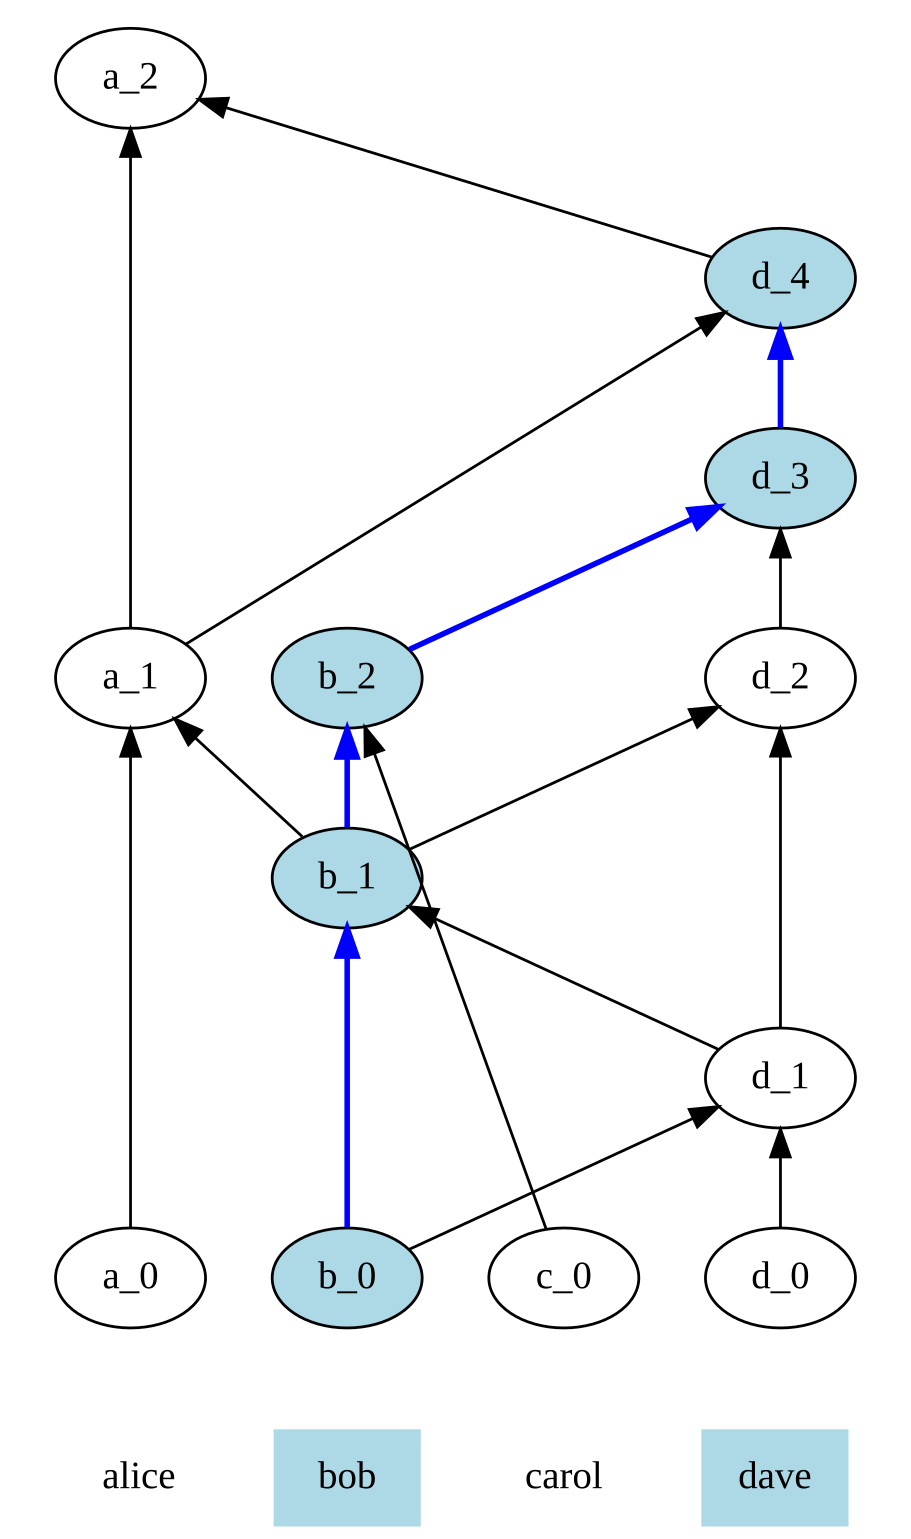
\includegraphics[width=.4\textwidth]{seen.png}
		}
		\ffigbox[\FBwidth]{%
			\caption{a\_1 strongly sees b\_0: it sees itself, b\_1 and d\_1, which are a
			supermajority and all see b\_0}
			\label{fig-stronglyseen}}{%
			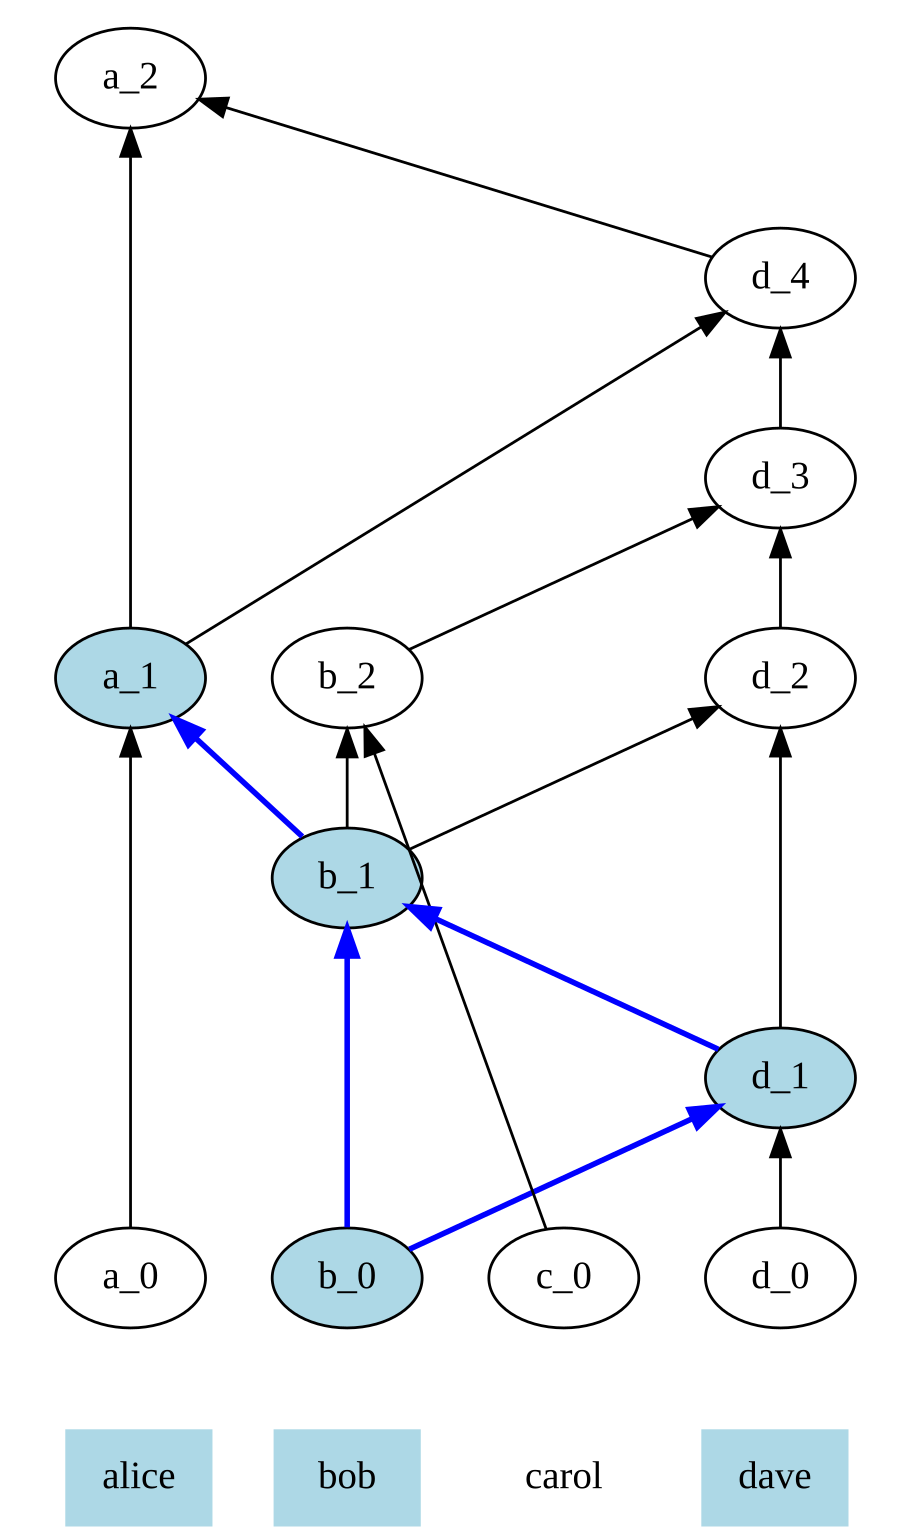
\includegraphics[width=.4\textwidth]{strongly_seen.png}
		}
	\end{floatrow}
\end{figure}

\subsection{General overview of the algorithm}

The nodes execute two main steps in an infinite loop:

\begin{itemize}
		\item Synchronise the gossip graph with another random node
		\item Determine whether any new blocks should be appended to the ordered set
\end{itemize}

\subsubsection{Synchronisation}

This step is responsible for building the gossip graph and spreading information around the
network. Nodes continually make random calls, called \emph{sync requests}, to other nodes and
exchange information about the graph, so that all correct nodes end up with the same data in their
graphs. The hashes and signatures in gossip events make sure that malicious nodes won't be able to
tamper with any part of the graph.

Whenever a node receives a sync request, it creates a new gossip event and sends a sync response
back. The self-parent of this event is the hash of the last gossip event created by the recipient,
and the other-parent is the hash of the last event created by the sender (which the recipient
learns about from the exchange). The recipient of the sync response also creates a new event with
analogous parents. Both events created also store the reason for which they were created (whether
due to a request, or a response).

If the recipient of a request/response believes it knows a network event that should be appended as
the next one in the chain, it records its vote as the payload of the newly created event. The other
nodes will learn of this vote during subsequent sync exchanges made by its creator.

\subsubsection{Determining order}

During this step, a node analyses the graph, counts the votes and decides which block should become
the next one. This step is a complex one and so it is described in detail in a separate subsection
below.

\subsection{Calculating the order}

To be able to order blocks, we need first to have some blocks that can be ordered.

As mentioned above, the gossip events may contain votes for network events. A gossip event which
sees events created by a supermajority of nodes that contain votes for a given network event is
said to \emph{see a valid block}, and we will call such gossip events \emph{block-votes}. The first
gossip event which strongly sees block-votes created by a supermajority of nodes is said to be an
\emph{observer}. The block-votes don't need to see the same valid block - in fact, it is the case
when they see different valid blocks that is the most interesting. However, they do have to only
refer to blocks that haven't been appended to the ordered set yet.

An observer implicitly carries a list of $N$ \emph{meta-votes}. Every meta-vote is just a binary
value denoting whether a corresponding node's block-vote is to be taken into account when
determining the order. An observer meta-votes $true$ on a node if it can strongly see a block-vote
by that node. Every node is being meta-voted on, hence there are $N$ meta-votes, and since an
observer strongly sees a supermajority of block-votes, by definition, at least $\frac{2}{3}N$ of
them are $true$.

Meta-votes reduce the problem of Byzantine agreement about the order to that of binary Byzantine
agreement, which has been solved previously\cite{aba}.

The algorithm described in \cite{aba} has some shortcomings, though, the most significant of which
is the need for a \emph{common coin}, a primitive which may require synchronicity and/or a trusted
third party for efficient creation or setup. The algorithm presented here works without such a
requirement.

\subsubsection{Binary agreement}

For the sake of simplicity, we will define the algorithm in terms of deciding a single
\emph{meta-election} - that is, deciding whether or not to take a single node's opinion into
account when trying to choose a single new block. We can view a meta-election for node $X$ with
latest agreed block $B$ as a function on a subset $H_{X,B}$ of the gossip graph $G$, which is the
set of all events that are descendants of any observer of this meta-election:

\[ \mathsf{meta\_election}_{X,B}: H_{X,B} \to \{0, 1, \bot\} \]

The $\bot$ value means that the result has not been decided yet at this point in the graph.

In order to calculate the meta-election value for events in $H_{X,B}$, we will need to calculate a
few helper values as well:

\begin{itemize}
	\item $\mathsf{stage}$ - a counter denoting the calculation stage
	\item $\mathsf{estimates}$ - a set of one or two values estimating the final result
	\item $\mathsf{bin\_values}$ - a helper set of binary values
	\item $\mathsf{aux}$ - a helper binary value
\end{itemize}

$\mathsf{stage}$ is an integer value which represents the stage of the protocol we are considering
when looking at a specific gossip event. A number is associated with each gossip event, such that
the $\mathsf{stage}$ of the observers is always 0. The $\mathsf{stage}$ of any other gossip event
is either the $\mathsf{stage}$ of its self-parent, or the stage of its self-parent plus one under 
specific conditions. The exact conditions under which the stage is incremented will be described
later in more details. Other variables such as $\mathsf{estimates}$, $\mathsf{bin\_values}$ and
$\mathsf{aux}$ all depend on the stage.

$\mathsf{estimates}$ is a set of binary values that represent the perceived opinion(s) of the
creator of any gossip event on the outcome of a meta-election. The $\mathsf{estimate}$ of an
observer is the set containing just its own meta-vote. The $\mathsf{estimate}$ of any subsequent
gossip event can be a different set as described below.

If the estimates for an event's self-parent contain a single value $v$, and that event sees more 
than $\frac{N}{3}$ events with $\neg v$ in their $\mathsf{estimates}$ (which means that at least
one honest node estimated $\neg v$), this opposite value gets added to its own $\mathsf{estimates}$
(so it will contain both true and false).

\[ \mathsf{est}: H_{X,B} \to 2^{\{0,1\}} \]
\[ \mathsf{est}(e) = \left\{ \begin{array}{ll}
	\{ v \} & \textrm{if there exists an ancestor $d$ of $e$} \\
	& \textrm{such that $v = \mathsf{meta\_election}(d) \neq \bot$} \\
	\{ w \} & \textrm{if $e$ is an observer with meta-vote $w$} \\
	\{ 0,1 \} & \textrm{if $\mathsf{est}(\mathsf{self\_par}(e)) = \{v\}$} \\
	& \textrm{and $e$ sees $\geq\frac{N}{3}$ events $x$}\\
	& \textrm{by different nodes such that} \\
	& \textrm{$\mathsf{stage}(x) = \mathsf{stage}(e)$ and $\neg v \in \mathsf{est}(x)$} \\
	\mathsf{next\_est}(\mathsf{self\_par}(e)) & \textrm{if $\mathsf{stage}(e) > 
		\mathsf{stage}(\mathsf{self\_par}(e))$} \\
	\mathsf{est}(\mathsf{self\_par}(e)) & \textrm{otherwise}
\end{array} \right. \]

$\mathsf{self\_par}(e)$ denotes $e$'s self-parent, and $\mathsf{next\_est}$ and will be defined
later, once we have defined more values related to the events.

Once an event can see a supermajority of events by different nodes which agree in their estimates,
this agreed estimate becomes an element of this event's $\mathsf{bin\_values}$. This set serves to
validate values proposed by other nodes - if they propose something we don't have in
$\mathsf{bin\_values}$, we will reject it, as we have no way to ensure its validity.

\[ \mathsf{bv}: H_{X,B} \to 2^{\{0,1\}} \]
\[ \mathsf{bv}(e)  =  \{ v: \begin{array}[t]{l} \textrm{there exist $> \frac{2}{3}N$ events $x$} \\
	\textrm{by different nodes such that} \\
	\textrm{$e$ sees $x$ and $\mathsf{stage}(e) = \mathsf{stage}(x)$ and $v \in \mathsf{est}(x)$}\}
\end{array}\]

If an event's parent has an empty $\mathsf{aux}$ value, and the event itself has non-empty
$\mathsf{bin\_values}$, it can propose a value to be agreed. This proposing is realised by having a
non-empty $\mathsf{aux}$ value. If $\mathsf{bin\_values}$ contains just one value, this value
becomes the $\mathsf{aux}$ value; otherwise, we can pick an arbitrary value, so we will pick true.
If the parent's value isn't empty, it becomes our value as well.

\[ \mathsf{aux}: H_{X,B} \to \{0, 1, \bot\} \]
\[ \mathsf{aux}(e) = \left\{ \begin{array}{ll}
	v & \textrm{if there exists an ancestor $d$ of $e$} \\
	& \textrm{such that $v = \mathsf{meta\_election}(d) \neq \bot$} \\
	\bot & \textrm{if $\mathsf{bv}(e) = \varnothing$} \\
	w & \textrm{if $\mathsf{bv}(e) = \{ w \}$} \\
	& \textrm{and $\mathsf{aux}(\mathsf{self\_par}(e)) = \bot$ } \\
	1 & \textrm{if $\mathsf{bv}(e) = \{ 0,1 \}$} \\
	& \textrm{and $\mathsf{aux}(\mathsf{self\_par}(e)) = \bot$ } \\
	\mathsf{aux}(\mathsf{self\_par}(e)) & \textrm{if $\mathsf{aux}(\mathsf{self\_par}(e))
		\neq \bot$}
\end{array}\right. \]

Whenever an event sees a supermajority of events with valid $\mathsf{aux}$ values, we perform the
gradient leadership based concrete coin protocol, which will lead either to deciding the final
agreed value, or updating the estimates and moving to the next stage.  

First, let us define some helper functions:

\[ \mathsf{supermajority\_valid\_aux}: H_{X,B} \to \{0,1\} \]
\[ \mathsf{supermajority\_valid\_aux}(e) = \begin{array}[t]{l}
	\textrm{$e$ sees a supermajority} \\
	\textrm{of events $x$ by different nodes} \\
	\textrm{such that $\mathsf{stage}(x) = \mathsf{stage}(e)$} \\
	\textrm{and $\mathsf{aux}(x) \in \mathsf{bv}(e)$}
\end{array} \]

\[ \mathsf{count\_aux}: H_{X,B} \times \{0, 1\} \to \mathbb{N} \]
\[ \mathsf{count\_aux}(e, v) = \begin{array}[t]{l}
	\textrm{number of events $x$ by different nodes such that} \\
	\textrm{$e$ sees $x$ and $\mathsf{stage}(x) = \mathsf{stage}(e)$} \\
	\textrm{and $\mathsf{aux}(x) \in \mathsf{bv}(e)$ and $\mathsf{aux}(x) = v$}
\end{array} \]

Now we can define how to determine a decided value:

\[ \mathsf{meta\_election}: H_{X,B} \to \{0, 1, \bot\} \]
\[ \mathsf{meta\_election}(e) = \left\{ \begin{array}{ll}
	v & \textrm{if there exists an ancestor $d$ of $e$} \\
	& \textrm{such that $v = \mathsf{meta\_election}(d) \neq \bot$} \\
	1 & \textrm{if $\mathsf{stage}(e) \equiv 0\;(\textrm{mod}\;3)$} \\
	& \textrm{and $\mathsf{count\_aux}(e, 1) > \frac{2}{3}N$} \\
	0 & \textrm{if $\mathsf{stage}(e) \equiv 1\;(\textrm{mod}\;3)$} \\
	& \textrm{and $\mathsf{count\_aux}(e, 0) > \frac{2}{3}N$} \\
	\bot & \textrm{otherwise}
\end{array} \right. \]

If an event sees a supermajority of valid $\mathsf{aux}$ values, but isn't able to decide, the next
event will mark the beginning of the next stage of the algorithm. This lets us finally define
$\mathsf{stage}$:

\[ \mathsf{stage}: H_{X,B} \to \mathbb{N} \]
\[ \mathsf{stage}(e) = \left\{ \begin{array}{ll}
	0 & \textrm{if $e$ is an observer} \\
	\mathsf{next\_stage}(\mathsf{self\_par}(e)) & \textrm{otherwise}
\end{array}\right. \]
\[ \mathsf{next\_stage}: H_{X,B} \to \mathbb{N} \]
\[ \mathsf{next\_stage}(e) = \mathsf{stage}(e) + \left\{ \begin{array}{ll}
	1 & \textrm{if $\mathsf{supermajority\_valid\_aux}(e)$} \\
	& \textrm{and $\mathsf{next\_est}(e) \neq \bot$} \\
	0 & \textrm{otherwise}
\end{array}\right.\]

We will also define two auxiliary values derived from $\mathsf{stage}$ - $\mathsf{step}$ and
$\mathsf{round}$. They will be more convenient than $\mathsf{stage}$ in the description below.

\[ \mathsf{round}: H_{X,B} \to \mathbb{N} \]
\[ \mathsf{round}(e) = \mathsf{stage}(e) / 3 \]

\[ \mathsf{step}: H_{X,B} \to \mathbb{N} \]
\[ \mathsf{step}(e) = \mathsf{stage}(e) - \mathsf{round}(e) \times 3 \]

Under this definition, the sequential stages $0,1,2,3,...$ will translate to round 0, step 0; round
0, step 1; round 0, step 2; round 1, step 0; etc.

If we don't decide in a stage, we need new estimates for the next one. This is being taken care of
by the three-step concrete coin protocol briefly mentioned before:

\begin{itemize}
	\item In any round in step 0, we decide true if we see a supermajority of true $\mathsf{aux}$
		values. If we see a supermajority of false values, we update the estimate to false. If we
		don't see any supermajority, we estimate true in the next step.
	\item In any round in step 1, we proceed analogously to above, but in the opposite way: if we
		see a supermajority of false $\mathsf{aux}$ values, we decide false; if we see a
		supermajority of true values, we estimate true; if we don't see any supermajority, estimate
		false.
	\item Step 2 of any round is a genuinely flipped concrete coin step. If we see a supermajority
		of agreeing $\mathsf{aux}$ values, we update our estimate to that value, otherwise we flip
		a concrete coin (described below) and update our estimate to that. We never decide in a
		coin step.
\end{itemize}

How first two points work with regards to deciding can be seen in the definition of
$\mathsf{meta\_election}$ above.  To calculate new estimates, we will define a $\mathsf{next\_est}$
function (which appeared already in the definition of $\mathsf{est}$):

\[ \mathsf{est\_true}: H_{X,B} \to \{0,1\} \]
\[ \mathsf{est\_true} = \begin{array}[t]{l}
	\textrm{[($\mathsf{step}(e) = 1$ or $\mathsf{step}(e) = 2$) and $\mathsf{count\_aux}(e, 1) 
		> \frac{2}{3}N$]} \\
	\textrm{or ($\mathsf{step}(e) = 0$ and $\mathsf{count\_aux}(e, 0) \leq \frac{2}{3}N$} \\
	\textrm{and $\mathsf{meta\_election}(e) = \bot$)}
\end{array} \]

\[ \mathsf{est\_false}: H_{X,B} \to \{0,1\} \]
\[ \mathsf{est\_false} = \begin{array}[t]{l}
	\textrm{[($\mathsf{step}(e) = 0$ or $\mathsf{step}(e) = 2$) and $\mathsf{count\_aux}(e, 0) 
		> \frac{2}{3}N$]} \\
	\textrm{or ($\mathsf{step}(e) = 1$ and $\mathsf{count\_aux}(e, 1) \leq \frac{2}{3}N$} \\
	\textrm{and $\mathsf{meta\_election}(e) = \bot$)}
\end{array} \]

\[ \mathsf{next\_est}: H_{X,B} \to 2^{\{0,1\}} \cup \{ \bot \} \]
\[ \mathsf{next\_est}(e) = \left\{ \begin{array}{ll}
	\{1\} & \textrm{if $\mathsf{est\_true}(e)$} \\
	\{0\} & \textrm{if $\mathsf{est\_false}(e)$} \\
	\{\mathsf{coin\_flip}(e)\} & \textrm{if $\mathsf{coin\_flip}(e) \neq \bot$} \\
	\bot & \textrm{otherwise}
\end{array} \right. \]

$\mathsf{coin\_flip}$ is a function that gives the result of the concrete coin flip. In order to
define it, we must first define the gradient of leadership and responsiveness threshold.

Let us call the following hash the \emph{round hash}:

\[ \mathsf{round\_hash}: H_{X,B} \to [0, 2^{256}) \]
\[ \mathsf{round\_hash}(e) = \mathsf{hash}( \mathsf{hash}(X), \mathsf{hash}(B),
	\mathsf{hash}(\mathsf{round}(e))) \]

The \emph{leadership index} of node $Y$ at gossip event $e$ will be its index on the list of all
nodes in the network, sorted by XOR-distance from $\mathsf{round\_hash}(e)$ (the XOR-distance being
simply $Y \oplus \mathsf{round\_hash}(e)$).

In order to get the result of the coin flip, we will look for the first gossip event by the node
with the leader index 0 that has an $\mathsf{aux}$ value in the current step, and take the least
significant bit of its hash. There is one caveat, though - the first leader might be dead and never
gossip such an event. We can never know for sure because of the asynchronicity assumption.

To get past that hurdle, we use the $\mathsf{responsiveness\_threshold}$, which is just an integer
function of $N$. This threshold will denote the number of gossip events caused by responses we will
allow ourselves to create before we use another leader - one whose event we see, and who has the
lowest leadership index.

Formally, it would look like this:

\[ \mathsf{ev\_waited}: H_{X,B} \to \mathbb{N} \]
\[ \mathsf{ev\_waited}(e) = \begin{array}{l}
	\\
	\\
	\left\{ \begin{array}{ll}
		0 & \textrm{if $\mathsf{supermajority\_valid\_aux}(e)$} \\
		& \textrm{and not} \\
		& \mathsf{supermajority\_valid\_aux}(p) \\
		1 + \mathsf{ev\_waited}(p) & \textrm{if $\mathsf{cause}(e) = response$} \\
		\mathsf{ev\_waited}(p) & \textrm{otherwise}
	\end{array}\right. \\
	\\
	\textrm{where $p = \mathsf{self\_par}(e)$}
\end{array}\]

The function $\mathsf{ev\_waited}$ counts how many events passed since the first one where we could
theoretically flip the coin. We can use this to check whether the first leader "timed out".

But first, we will define a function that gives us the first event by a node which has an
$\mathsf{aux}$ value:

\[ \mathsf{first\_aux}: \mathcal{N} \times H_{X,B} \to H_{X,B} \cup \{ \bot \} \]
\[ \mathsf{first\_aux}(Y, e) = \begin{array}[t]{l}
	\textrm{the event $x$ created by Y such that $e$ sees $x$} \\
	\textrm{and $\mathsf{aux}(x) \neq \bot$ and $\mathsf{aux}(\mathsf{self\_par}(x)) = \bot$} \\
	\textrm{and $\mathsf{stage}(e) = \mathsf{stage}(x)$ if it exists; $\bot$ otherwise}
\end{array} \]

Let us denote the first leader by $L$. Then the function that tells us if the "timeout" happened
will be:

\[ \mathsf{leader\_timed\_out}: H_{X,B} \to \{0,1\} \]
\[ \mathsf{leader\_timed\_out}(e) = \begin{array}[t]{l}
	\textrm{$\mathsf{first\_aux}(L, e) = \bot$ and} \\
	\mathsf{ev\_waited}(e) > \mathsf{responsiveness\_threshold}(N)
\end{array} \]

The event that generates the coin will be calculated the following way:

\[ \mathsf{coin\_event}: H_{X,B} \to H_{X,B} \cup \{ \bot \} \]
\[ \mathsf{coin\_event}(e) = \left\{ \begin{array}{ll}
	\mathsf{first\_aux}(L, e) & \textrm{if not $\mathsf{leader\_timed\_out}(e)$} \\
	\mathsf{first\_aux}(Y, e) & \textrm{if $\mathsf{leader\_timed\_out}(e)$,}\\
	& \textrm{where $Y$ is the node with} \\
	& \textrm{the lowest leadership index} \\
	& \textrm{for which $\mathsf{first\_aux}(Y, e) \neq \bot$} \\
	\bot & \textrm{otherwise}
\end{array}\right. \]

Then, the coin flip will be just:

\[ \mathsf{coin\_flip}: H_{X,B} \to \{0,1,\bot\} \]
\[ \mathsf{coin\_flip}(e) = \left\{ \begin{array}{ll}
	\textrm{lowest order bit} & \\
	\textrm{of $\mathsf{hash}(\mathsf{coin\_event}(e))$} & \textrm{if $\mathsf{coin\_event}(e)
		\neq \bot$} \\
	\bot & \textrm{otherwise}
\end{array}\right. \]

We call the result of the $\mathsf{coin\_flip}$ function a \emph{genuinely flipped concrete coin}.

This is all we need to reach consensus on the meta-votes.

\subsubsection{Agreement about the next block}

Using the above, every node can calculate the results of all meta-elections. Once the results are
known, they can be used to determine the next block in the ordered set.

Let us remember that the meta-elections started with a set of observers - a set of events that all
strongly see a supermajority of block-votes. The results of the meta-elections tell us which
block-votes are to be taken into account.

The properties of meta-elections ensure that all nodes will agree on the considered set of nodes.
What we need to do is change that into an agreement on what the next block should be. This is
pretty trivial, although we must consider two issues: every node could create multiple block-votes,
and every block-vote could see multiple valid blocks.

To counter the first issue, we can just take the earliest block-vote created by a given node. The
events created by a single node form a linear sequence, so the earliest one is well-defined. This
narrows the considered set down to a single block-vote per node.

The next step is to choose a valid block among potentially multiple ones seen by the chosen
block-vote. To do that, we can take the lexicographically first one, or use really any method that
will always choose the same element of a set.

Once we have one vote on a block per node, we just count them and the next agreed block will be the
one with the most votes. Any ties can be broken again by lexicographic ordering, or some other
method.

This completes the description of the algorithm. The next section will prove that it is correct,
that is, that it provides robust consensus in an asynchronous setting, and in the presence of
Byzantine faults.

\section{Proof of correctness}

Let us begin by stating two important properties of the gossip graph.

\begin{defn}
	We call two gossip graphs \emph{consistent} iff for every gossip event $x$ that is present in
	both graphs, both contain the same set of ancestors of $x$ with the same sets of edges between
	them.
\end{defn}

\begin{lem}\label{consistency}
	All nodes in the network have consistent gossip graphs.
\end{lem}

\begin{lem}\label{stronglysee}
	If a pair of gossip events $(x,y)$ is a fork, and another gossip event $z$ strongly sees $x$,
	then no other gossip event in a consistent graph can strongly see $y$.
\end{lem}

We won't prove the above lemmas - they have been proved in \cite{hg} (as Lemma 5.11 and 5.12,
respectively).

Let us now prove some properties of our approach stemming from it being an adaptation of
\cite{aba}.

\begin{lem}[Progress]\label{progress}
	If a correct node created a gossip event in stage $s$, every other correct node will eventually
	create an event in stage $s$ as well.
\end{lem}

\begin{proof}
	Step numbers are based on seeing a supermajority of some events - either events seeing a valid
	block (for observers, stage 0), or events in the previous stage having valid $\mathsf{aux}$
	values (stage greater than 0). Assume there is event $e$ in stage $s$ created by a correct node
	- it means that it sees a set of events that allowed it to proceed to stage $s$. A correct node
	will continue gossiping, so every other correct node will eventually learn of $e$ and create a
	descendant of $e$.

	A descendant of $e$ sees everything that $e$ sees (provided that $e$ is not a part of a fork -
	but its creator is correct, so it is not). If $e$ was in stage 0, any descendant will thus
	automatically be in stage at least 0.

	Assume that the lemma is true for stage $s-1$. $e$ has a self-ancestor in stage $s-1$, which
	means that every correct node will eventually create an event in stage $s-1$. Any later event
	which has $e$ as an ancestor will thus have an event in stage $s-1$ as a self-ancestor, and
	will see events allowing it to progress to stage $s$. Thus, the lemma is also true for $s$. By
	induction, the proof is complete.
\end{proof}

\begin{lem}\label{common}
	The probability that the genuinely flipped concrete coin is common and pseudorandom is
	$> \frac{2}{3} - \varepsilon$, with an arbitrarily small $\varepsilon$ when the responsiveness
	threshold is sufficiently high, and the required threshold value is logarithmic in $N$.
\end{lem}

\begin{proof}
	First, note that the node with leadership index 0 is common and pseudorandom. It is common, 
	as the nodes share the list of the nodes in the network, the last decided block in the ordered
	set and the round number. It is pseudorandom, as it is based on a cryptographic hash of values
	outside the nodes' control.

	With probability $> \frac{2}{3}$, the node with leadership index 0 will be honest. In such a
	case, it gossips its events honestly to random nodes, so that correct nodes will receive the
	coin event before "timeout" with probability $p$, which is close to 1.

	The probability of the coin being common and random is strictly larger than the probability of 
	the event described above. Such an event's probability, on the other hand, is $> \frac{2}{3}p$.
	As long as $p > 1 - \frac{3}{2}\varepsilon$, this is $> \frac{2}{3} - \varepsilon$. $p > 
	1 - \frac{3}{2}\varepsilon$ can be ensured by choosing the right responsiveness threshold. In
	fact, $p$ can be arbitrarily close to 1 with a large enough responsiveness threshold.

	Since gossip from correct nodes is expected to reach everyone in $O(\log{N})$ exchanges, the
	minimal responsiveness threshold will also be logarithmic in $N$.
\end{proof}

\begin{lem}\label{claima}
	If all correct nodes created events in stage $s \equiv 2\;(\textrm{mod}\;3)$ (step 2), and no
	such event decided a value, then the estimates of their events in the next stage will be in
	agreement with probability $> \frac{1}{3} - \varepsilon'$ for arbitrarily small
	$\varepsilon'$.
\end{lem}

\begin{proof}
	The estimate in a stage after the coin stage is based on the auxiliary values seen by events
	in the coin stage. There are five possible situations here:

	\begin{itemize}
			\item All correct nodes' events in stage $s+1$ see a supermajority of $true$ values
				from stage $s$ - estimates agree with probability 1.
			\item All correct nodes' events in stage $s+1$ see a supermajority of $false$ values
				from stage $s$ - estimates agree with probability 1.
			\item Some correct nodes' events in stage $s+1$ see a supermajority of $true$ values
				from stage $s$; the others throw a coin, which is common and random with
				probability $> \frac{2}{3}-\varepsilon$, and the result is $true$ with probability 
				$\frac{1}{2}$ - estimates agree with probability $> \frac{1}{3} - \varepsilon'$
				(where $\varepsilon' = \frac{1}{2}\varepsilon$).
			\item Some correct nodes' events in stage $s+1$ see a supermajority of $false$ values
				from stage $s$; the others throw a coin, which is common and random with
				probability $> \frac{2}{3}-\varepsilon$, and the result is $false$ with probability 
				$\frac{1}{2}$ - estimates agree with probability $> \frac{1}{3} - \varepsilon'$.
			\item No correct nodes' events in stage $s+1$ see a supermajority of any value in stage
				$s$; all of them throw a coin, which is common and random with probability
				$> \frac{2}{3} - \varepsilon$ - estimates agree with probability $> \frac{2}{3} -
				\varepsilon$.
	\end{itemize}

	The total probability of agreement is a weighted average of five values, all greater than
	$\frac{1}{3} - \varepsilon'$, which means the total probability is also greater than
	this value.
\end{proof}

\begin{lem}\label{claimb}
	If all correct nodes' first events in stage $s$ had $\mathsf{estimates} = \{v\}$, their first
	events in stage $s+1$ will also have $\mathsf{estimates} = \{v\}$.
\end{lem}

\begin{proof}
	If all correct nodes only estimate $v$, there is no way for any event to see even $\frac{N}{3}$
	of estimates for $\neg v$ - so no event by a correct node will have it in its estimates in
	stage $s$.

	For a value to be an element of $\mathsf{bin\_values}$, there must be a supermajority of events
	estimating that value. Because of the above, the only value that can have a supermajority is
	$v$. Thus, every event with nonempty $\mathsf{bin\_values}$ will have it equal to $\{v\}$.
	Hence, every event with an $\mathsf{aux}$ value will have it equal to $v$.

	In order to proceed to the next stage, an event has to see a supermajority of valid
	$\mathsf{aux}$ values. No event can have a value other than $v$ as $\mathsf{aux}$ in stage $s$,
	so there will always be a supermajority for $v$. Depending on the stage number, this can either
	lead to deciding $v$, or estimating $v$ in stage $s+1$. Either way, the agreement will still
	hold.
\end{proof}

\begin{lem}\label{decide}
	If all correct nodes' first events in round $r$ had $\mathsf{estimates} = \{v\}$, they will all
	decide $v$ within round $r$.
\end{lem}

\begin{proof}
	No matter what malicious nodes do, there is less than a third of them, so no event by a correct
	node will have $\neg v$ in estimates (by definition of the $\mathsf{est}$ function). This means
	that for $\mathsf{bin\_values}$ of an event to be non-empty, it must see a supermajority of
	estimates for $v$, as there will never be a supermajority for $\neg v$.

	The above means that no correct node will add $\neg v$ to $\mathsf{bin\_values}$, so all of
	them will eventually create an event with $\mathsf{aux} = v$. This means there will be a
	supermajority of events by different creators with $\mathsf{aux} = v$, which will make the
	correct nodes either decide at step 0 (if $v = 1$), or estimate 0 for the next step and
	decide then.
\end{proof}

\begin{thm}[Binary Byzantine Consensus]\label{binconsensus}
	The algorithm for calculating meta-election results presented in this paper satisfies the
	general properties of a Byzantine fault tolerant consensus algorithm:
	\begin{itemize}
		\item \emph{Validity} - if a correct node decides on a value, it has been proposed by a
			correct node.
		\item \emph{Agreement} - if a correct node decides on a value, all correct nodes decide
			on that value.
		\item \emph{Integrity} - once a correct node decides on a value, it never decides on
			another value.
		\item \emph{Termination} - all correct nodes eventually decide with probability 1.
	\end{itemize}
\end{thm}

\begin{proof}[Validity]
	We will prove an equivalent statement: that if initially all correct nodes propose $v$, then
	all correct nodes will decide $v$. Since $v$ is a binary value, a node can only decide a value
	not proposed by a correct node if all correct nodes propose $v$, and the node decides $\neg v$.
	Thus, deciding $v$ when all correct nodes propose $v$ is equivalent to always deciding on a
	value proposed by a correct node.

	If all correct nodes propose $v$, they will all put $v$ in their estimates. By Lemma
	\ref{decide}, they will all decide $v$ within the first round.
\end{proof}

\begin{proof}[Agreement]
	Assume there is an event $e$ created by a correct node which was able to decide a value $v$. It 
	means that $\mathsf{step}(e) = 0$ or $\mathsf{step}(e) = 1$ (there would be no decision
	otherwise). This event must have seen a supermajority of events with $\mathsf{aux} = v$, which
	means there was no supermajority for $\neg v$. Thus, if a correct node has seen a supermajority
	in this stage, it must have been for $v$, so it would decide $v$. If it wasn't, it would
	estimate $v$ for the next stage, which means there will be agreement at the start of the next
	stage. Following Lemma \ref{claimb}, this agreement will propagate to the end of the stage and
	the next stage, until everyone decides $v$.
\end{proof}

\begin{proof}[Integrity]
	Once an event $e$ created by a correct node decides on a value $v$, all later events created by
	that node will have event $e$ as an ancestor. Following the definition of
	$\mathsf{meta\_election}$, all later events will also decide $v$.
\end{proof}

\begin{proof}[Termination]
	By Lemma \ref{progress}, if a correct node creates an event in stage $s$, then every correct
	node eventually creates an event in stage $s$. This means there will be events by 
	$> \frac{2}{3}N$ correct nodes, which will eventually be seen by every correct node.  Every
	such event will have non-empty estimates. It is not possible for both 0 and 1 to be estimated
	by $< \frac{N}{3}$ events by different correct nodes, so at least one of those values will
	eventually be an element of estimates of every correct node's event.
	
	Eventually, the events with agreeing estimates will all be seen by an event created by every
	correct node. Hence, every correct node will eventually create an event with non-empty
	$\mathsf{bin\_values}$, and so an $\mathsf{aux}$ value.

	The events with $\mathsf{aux}$ values will eventually be seen by every correct node's event,
	which means every correct node will eventually either decide or progress to the next stage.

	By Lemma \ref{claima}, if no node decided in step 0 or 1, they will all agree after step 2 with
	probability $> \frac{1}{3} - \varepsilon'$. By Lemma \ref{decide}, this means they will decide
	in the next round with probability $> \frac{1}{3} - \varepsilon'$. Thus, the probability of no
	agreement in round $r$ is $< \left( 1 - \frac{1}{3} + \varepsilon' \right)^4 < 
	\left(\frac{2}{3} + \varepsilon'\right)^r$. This tends to 0 as $r$ increases, so the nodes will
	eventually decide with probability 1.
\end{proof}

The above theorem proves that our algorithm will reach agreement about every single meta-election
in a Byzantine fault tolerant way. This is not the end, though - we also need to prove that
meta-elections lead to agreement about the next block in the ordered set. The proof of that is
presented below.

\begin{lem}\label{minvotes}
	If the result of a meta-election is $v$, there have been at least $\frac{N}{3}$ meta-votes for
	$v$.
\end{lem}

\begin{proof}
	Assume there have been less than $\frac{N}{3}$ meta-votes for $v$ and $v$ has been decided.
	When nodes that initially meta-voted $v$ create an event that sees a supermajority of
	meta-votes, this supermajority must contain at least $\frac{N}{3}$ votes for $\neg v$ - so
	their estimates will contain $\neg v$. On the other hand, no node that meta-voted $\neg v$ can
	ever create an event that will see at least $\frac{N}{3}$ estimates for $v$, so they won't add
	$v$ to estimates.

	Due to the above, any supermajority among the estimates must be for $\neg v$. Any event with
	non-empty $\mathsf{bin\_values}$ can thus only have $\neg v$ in this set, which means that
	all valid $\mathsf{aux}$ values will also be $\neg v$, which will lead to a decision on $\neg
	v$ within two stages.

	This is a contradiction. Such a situation is impossible, which proves the lemma.
\end{proof}

\begin{lem}\label{nonempty}
	The set of nodes for which the result of meta-election is $true$ is always non-empty.
\end{lem}

\begin{proof}
	Assume all meta-elections resulted in $false$. By Lemma \ref{minvotes}, at least $\frac{N}{3}$
	nodes meta-voted $false$ for every node, so there have been at least $\frac{N^2}{3}$ meta-votes
	for $false$.

	On the other hand, by definition of an observer, every node voted $true$ for more than
	$\frac{2}{3}N$ nodes - so there have been more than $\frac{2}{3}N^2$ meta-votes for $true$,
	which leaves less than $\frac{N^2}{3}$ meta-votes for $false$ (there are $N^2$ meta-votes in
	total: $N$ nodes meta-vote in $N$ meta-elections).

	This is a contradiction, which proves the lemma.
\end{proof}

\begin{thm}[Byzantine Consensus]
	The algorithm for calculating the next block presented in this paper satisfies the general
	properties of a Byzantine fault tolerant consensus algorithm:
	\begin{itemize}
		\item \emph{Validity} - if a correct node decides on a value, it has been proposed by a
			correct node.
		\item \emph{Agreement} - if a correct node decides on a value, all correct nodes decide
			on that value.
		\item \emph{Integrity} - once a correct node decides on a value, it never decides on
			another value.
		\item \emph{Termination} - all correct nodes eventually decide with probability 1.
	\end{itemize}
\end{thm}

\begin{proof}[Validity]
	Assume a correct node decided that the next block should be a block $B$ containing a network
	event $E$. For such a situation to happen, there must have been a block-vote for $B$, and such
	a block-vote must have seen a supermajority of votes for $E$. A supermajority will always
	contain a correct node, so a correct node must have voted for $E$.
\end{proof}

\begin{proof}[Agreement]
	Assume that a correct node decided the next block $B$. Since a decision has been reached, this
	means that there is consensus about the meta-votes, so every correct node will have chosen the
	same nodes' block-votes. 

	For any observer to meta-vote $true$ on a node, it must have strongly seen a block-vote by that
	node. By Lemma \ref{stronglysee}, even if that node created a fork, if any other observers also
	voted $true$ on that node, they must have strongly seen block-votes on the same fork. Thus, we
	can consider block-votes by all elected nodes to form linear histories - which will be seen the
	same way by all nodes by Lemma \ref{consistency}.

	In a linear history, the earliest block-vote is well-defined. Also, because all correct nodes
	see the same history, they will all choose the same block-vote as the earliest. If the
	block-vote votes for multiple blocks, all correct nodes will use the same tie-breaker algorithm
	and choose the same single one. Thus, all correct nodes will gather the same set of votes, and
	because they use the same voting rules, decide the same block as the next one.
\end{proof}

\begin{proof}[Integrity]
	By construction of the algorithm, once the next block has been decided, it is appended to the
	ordered set and no other block can be decided in its place.
\end{proof}

\begin{proof}[Termination]
	For every network event, we expect all correct nodes to eventually vote for it. This means
	there will be a supermajority of votes for every event, which will eventually be seen by some
	other events - block-votes - created by each correct node. The block-votes will eventually be
	strongly seen by other events created by each correct node - the observers. Once there is a
	supermajority of observers, we start the binary agreement algorithm, which will terminate
	by Theorem \ref{binconsensus}. After binary agreement terminates, because the set of voters for
	the next block is non-empty (by Lemma \ref{nonempty}), the next block is already determined -
	so the agreement about the next block also terminates.
\end{proof}

\section{Conclusions}

A new consensus algorithm has been presented, building upon some previous achievements in this
field (\cite{hg}, \cite{aba}, \cite{trivial}), but combining their features in a novel way. It is
asynchronous (as in \cite{hg} and \cite{aba}), uses a gossip graph (as in \cite{hg} and
\cite{snowflake}), and generates randomness, which is necessary for asynchronous consensus
\cite{flp}, using a concrete coin (as in \cite{trivial}). We believe this approach will be useful
in numerous applications, one of which is the SAFE Network.

\label{references}

\begin{thebibliography}{4}

\bibitem{hg} Baird L. \textit{The Swirlds Hashgraph Consensus Algorithm: Fair, Fast, Byzantine
	Fault Tolerance}, Swirlds Tech Report SWIRLDS-TR-2016-01 (2016)

\bibitem{aba} Mostefaoui A., Hamouna M., Raynal M. \textit{Signature-Free Asynchronous Byzantine
	Consensus with $t < n/3$ and $O(n^2)$ Messages}, ACM PODC (2014)

\bibitem{trivial} Micali S. \textit{Byzantine Agreement, Made Trivial}, (2018)

\bibitem{hbbft} Miller A., Xia Y., Croman K., Shi E., Song D. \textit{The Honey Badger of BFT
	Protocols}, CCS (2016)

\bibitem{snowflake} Team Rocket \textit{Snowflake to Avalanche: A Novel Metastable Consensus
	Protocol Family for Cryptocurrencies}, (2018)

\bibitem{flp} Fischer M. J., Lynch N. A., Paterson M. S. \textit{Impossibility of Distributed
	Consensus with One Faulty Process}, JACM Vol. 32 Issue 2 (April 1985)

\end{thebibliography}

\end{document}
